% Current vs proposed operator workflow (Section 1.2).
\documentclass[tikz,border=1pt]{standalone}
% =====================================================================
%  Shared style for every diagram in the proposal.
%  Each figure is a standalone TikZ file that \input's this preamble, so
%  all diagrams use the same font family (Computer Modern, T1 -- identical
%  to the LLNCS body text), the same sizes and the same palette.
%
%  Font rule (do not change per figure):
%    node text   \footnotesize  (8 pt)
%    edge labels \scriptsize    (7 pt)
%    titles      \footnotesize\bfseries
%  Figures are drawn at their final width (<= 12.2 cm, the LLNCS text
%  width) and included WITHOUT scaling, so the printed size is the same
%  in every figure.
% =====================================================================
\usepackage[T1]{fontenc}
\usepackage{amsmath,amssymb}
\usepackage{xcolor}
\usepackage{tikz}
\usetikzlibrary{positioning,arrows.meta,shapes.geometric,shapes.multipart,
  fit,backgrounds,calc,shadows,patterns}

% ---- palette ---------------------------------------------------------
\definecolor{cBlue}{HTML}{0B4F8A}    % application / API
\definecolor{cOrange}{HTML}{B4540A}  % processing / services
\definecolor{cPurple}{HTML}{5B3CC4}  % data stores
\definecolor{cGreen}{HTML}{1B7A3A}   % success / output
\definecolor{cRed}{HTML}{B42318}     % error / risk
\definecolor{cGray}{HTML}{5F6672}    % external / neutral
\definecolor{cInk}{HTML}{1F2933}     % text and arrows

\colorlet{fBlue}{cBlue!9}
\colorlet{fOrange}{cOrange!10}
\colorlet{fPurple}{cPurple!9}
\colorlet{fGreen}{cGreen!10}
\colorlet{fRed}{cRed!9}
\colorlet{fGray}{cGray!8}

% ---- fonts -----------------------------------------------------------
\newcommand{\figfont}{\footnotesize}
\newcommand{\lblfont}{\scriptsize}
\newcommand{\code}[1]{\texttt{#1}}

\tikzset{
  every picture/.style={font=\figfont, line join=round, >={Stealth[length=4pt,width=3.4pt]}},
  every node/.append style={execute at begin node={\hyphenpenalty=10000\exhyphenpenalty=10000}},
  base/.style={draw, rounded corners=2pt, line width=0.6pt, align=center,
               inner xsep=3pt, inner ysep=2.5pt, text=cInk, font=\figfont},
  app/.style={base, draw=cBlue, fill=fBlue},
  svc/.style={base, draw=cOrange, fill=fOrange},
  data/.style={base, draw=cPurple, fill=fPurple},
  ok/.style={base, draw=cGreen, fill=fGreen},
  bad/.style={base, draw=cRed, fill=fRed},
  ext/.style={base, draw=cGray, fill=fGray},
  plain/.style={base, draw=none, fill=none},
  db/.style={cylinder, shape border rotate=90, aspect=0.22, draw=cPurple,
             fill=fPurple, line width=0.6pt, align=center, text=cInk,
             minimum height=9mm, font=\figfont},
  decision/.style={diamond, aspect=2.2, draw=cOrange, fill=fOrange,
                   line width=0.6pt, align=center, inner sep=1pt, text=cInk, font=\figfont},
  actor/.style={draw=cInk, fill=fGray, line width=0.8pt, rounded corners=0pt,
                align=center, inner sep=3pt, font=\figfont\bfseries},
  layer/.style={draw=cGray!60, fill=cGray!4, rounded corners=3pt, line width=0.5pt},
  layertitle/.style={font=\lblfont\bfseries, text=cGray, anchor=north west, inner sep=2pt},
  arr/.style={->, draw=cInk, line width=0.6pt},
  darr/.style={->, draw=cGray, line width=0.6pt, dashed},
  biarr/.style={<->, draw=cInk, line width=0.6pt},
  lbl/.style={font=\lblfont, text=cInk, inner sep=1.5pt},
  lblbg/.style={font=\lblfont, text=cInk, inner sep=1.5pt, fill=white},
}

% ---- UML sequence-diagram helpers -----------------------------------
%  \lifeline{id}{x}{label}{bottom y}   head box + dashed life line
%  \msg{x1}{x2}{y}{label}              synchronous call (solid)
%  \ret{x1}{x2}{y}{label}              reply (dashed)
%  \selfmsg{x}{y}{label}               call to self, label on the right
%  \fragment{kind}{guard}{x1}{y1}{x2}{y2}  combined fragment (alt/loop/par)
\newcommand{\lifeline}[4]{%
  \node[app, text width=19mm, minimum height=8.5mm, font=\figfont\bfseries] (#1) at (#2,0) {#3};
  \draw[cGray, dashed, line width=0.5pt] (#1.south) -- (#2,#4);}
\newcommand{\msg}[4]{%
  \draw[arr] (#1,#3) -- node[lbl, above] {#4} (#2,#3);}
\newcommand{\ret}[4]{%
  \draw[darr] (#1,#3) -- node[lbl, above] {#4} (#2,#3);}
\newcommand{\selfmsg}[3]{%
  \draw[arr] (#1,#2+0.12) -- ++(0.3,0) -- ++(0,-0.24) -- ++(-0.3,0);
  \node[lbl, anchor=west, align=left] at (#1+0.35,#2) {#3};}
\newcommand{\fragment}[6]{%
  \draw[cGray, line width=0.5pt] (#3,#4) rectangle (#5,#6);
  \node[anchor=north west, draw=cGray, fill=white, font=\lblfont\bfseries,
        inner sep=1.5pt, line width=0.5pt] at (#3,#4) {#1};
  \if\relax\detokenize{#2}\relax\else
  \node[anchor=north west, font=\lblfont, text=cGray, inner sep=1.5pt] at (#3+0.75,#4) {[#2]};\fi}
\newcommand{\activation}[3]{% x, y top, y bottom
  \draw[draw=cBlue, fill=fBlue, line width=0.5pt] (#1-0.07,#2) rectangle (#1+0.07,#3);}

\begin{document}
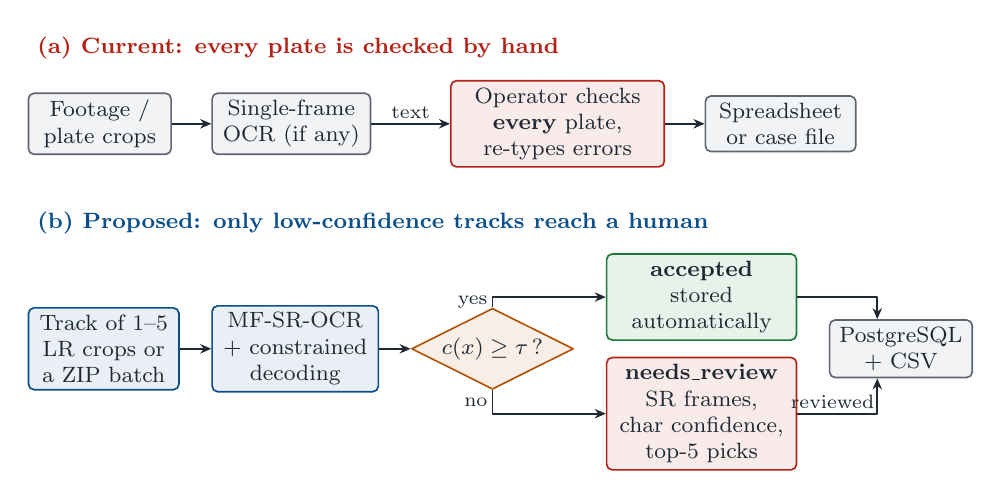
\begin{tikzpicture}[node distance=5mm and 5mm]
  % ---------------- (a) current ----------------
  \node[font=\figfont\bfseries, text=cRed, anchor=west] (ta) at (0,0)
    {(a) Current: every plate is checked by hand};
  \node[ext, text width=16mm, below=3mm of ta.south west, anchor=north west] (a1)
    {Footage /\\plate crops};
  \node[ext, text width=18mm, right=5mm of a1] (a2) {Single-frame\\OCR (if any)};
  \node[bad, text width=25mm, right=10mm of a2] (a3)
    {Operator checks\\\textbf{every} plate,\\re-types errors};
  \node[ext, text width=17mm, right=5mm of a3] (a4) {Spreadsheet\\or case file};
  \draw[arr] (a1) -- (a2);
  \draw[arr] (a2) -- node[lbl, above] {text} (a3);
  \draw[arr] (a3) -- (a4);

  % ---------------- (b) proposed ----------------
  \node[font=\figfont\bfseries, text=cBlue, anchor=north west] (tb)
    at ([yshift=-6mm]a1.south west)
    {(b) Proposed: only low-confidence tracks reach a human};
  \node[app, text width=17mm, below=8mm of tb.south west, anchor=north west] (b1)
    {Track of 1--5\\LR crops or\\a ZIP batch};
  \node[app, text width=19mm, right=4mm of b1] (b2)
    {MF-SR-OCR\\+ constrained\\decoding};
  \node[decision, aspect=2, right=4mm of b2] (b3) {$c(x)\ge\tau$\,?};
  \node[ok, text width=22mm, above right=1mm and 4mm of b3.east, anchor=south west] (b4)
    {\textbf{accepted}\\stored automatically};
  \node[bad, text width=22mm, below right=1mm and 4mm of b3.east, anchor=north west] (b5)
    {\textbf{needs\_review}\\SR frames,\\char confidence,\\top-5 picks};
  \node[ext, text width=16mm, anchor=west] (b6) at ([xshift=4mm]b4.east |- b3)
    {PostgreSQL\\+ CSV};
  \draw[arr] (b1) -- (b2);
  \draw[arr] (b2) -- (b3);
  \draw[arr] (b3.north) |- node[lbl, pos=0.25, left] {yes} (b4.west);
  \draw[arr] (b3.south) |- node[lbl, pos=0.25, left] {no} (b5.west);
  \draw[arr] (b4.east) -| ([xshift=-3mm]b6.north);
  \draw[arr] (b5.east) -| node[lbl, pos=0.22, above] {reviewed} ([xshift=-3mm]b6.south);
\end{tikzpicture}
\end{document}
